Bayesian Optimization is a optimization algorithm that uses a probabilistic model to approximate the objective function \textit{(surrogate model)} and uses this model to guide the search for the optimal solution. The general procedure can be described as follows:
\begin{enumerate}
    \item choose surrogata function that approximate the real objective function (prior)
    \item repeat until stopping condition
          \begin{enumerate}
              \item given a number of observations (computed from the real objective function), update the surrogate function (posterior distribution). Default choice is usually a Gaussian Process
              \item optimize a cheap \textit{acquisition function / utility function} based on the posterior distribution to find the new point to sample. Also has the responsability of balancing exploration and exploitation
          \end{enumerate}
\end{enumerate}

\paragraph*{Choice of Prior}
In this lab, we'll use three different prior distribution to sample the initial points for the optimization algorithm. The three distributions are:
\begin{itemize}
    \item \textit{Prior1}: Uniform in the range $[0, 1]$
    \item \textit{Prior2}: Uniform in the range $[0, 0.5]$
    \item \textit{Prior3}: Uniform in the range $[0.5, 1]$
\end{itemize}
\begin{table}[H]
    \centering
    \begin{tabular}{|c|c|c|}
        \textbf{Prior} & \textbf{Mean}  & \textbf{Std. Deviation} \\\hline
        Prior1         & 0.9967, 1.0966 & 0.0026, 0.0198          \\
        Prior2         & 0.9963, 1.0999 & 0.0043, 0.0206          \\
        Prior3         & 0.6991, 0.7897 & 0.4528, 0.4687          \\
        \hline
    \end{tabular}
    \caption{Best point found with Objective1 and UCB acquisition function}
    \label{tab:prior}
\end{table}
We can see that Prior3 achieves worse results due to the fact that the prior distribution doesn't cover the optimal region. In particular the standard deviation is very high, which means tha the Bayesian Optimzation found good solutions in some cases but it's not consistent.

\begin{figure}[H]
    \begin{subfigure}{0.5\textwidth}
        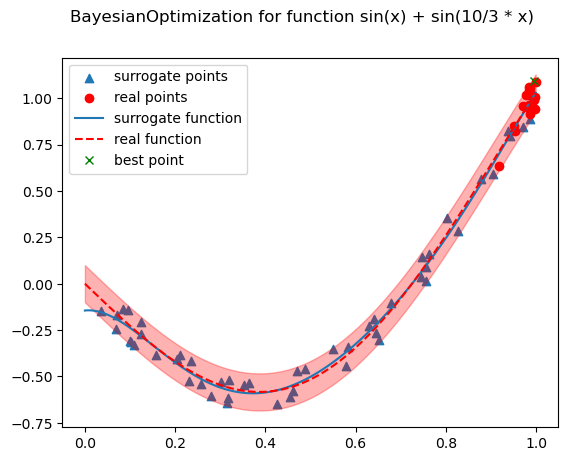
\includegraphics[width=\textwidth]{lab6/imgs/obj1_pr1.png}
        \caption{Prior1}
    \end{subfigure}
    \begin{subfigure}{0.5\textwidth}
        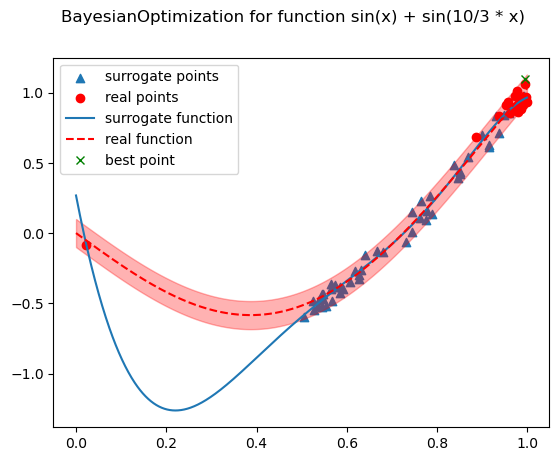
\includegraphics[width=\textwidth]{lab6/imgs/obj1_pr2.png}
        \caption{Prior2}
    \end{subfigure} \\
    \begin{subfigure}{\textwidth}
        \centering
        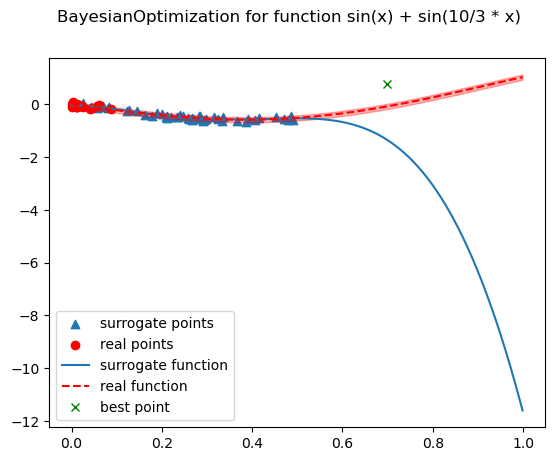
\includegraphics[width=0.5\textwidth]{lab6/imgs/obj1_pr3.png}
        \caption{Prior3}
    \end{subfigure}
    \caption{Objective1 with different prior distribution}
    \label{fig:bo-prior}
\end{figure}
It's also interesting to note how the Gaussian Process differently approximate the real objective function based on the prior distribution: Prior1 better approximates the real function since it covers the entire range of the function.

\paragraph*{Acquisition Function}
\begin{table}[H]
    \centering
    \begin{tabular}{|c|c|c|}
        \textbf{Prior} & \textbf{Mean}  & \textbf{Std. Deviation} \\\hline
        UCB            & 0.9715, 1.5490 & 0.0055, 0.0202          \\
        LCB            & 0.9688, 1.5527 & 0.0070, 0.0297          \\
        PI             & 0.9661, 1.5107 & 0.0101, 0.0556          \\
        EI             & 0.9693, 1.4752 & 0.0142, 0.0649          \\
        \hline
    \end{tabular}
    \caption{Best point found with Objective1 and UCB acquisition function}
    \label{tab:acquisition}
\end{table}
The results are roughlu the same for all the acquisition functions, with EI slightly worse than the others.

\begin{figure}[H]
    \begin{subfigure}{0.5\textwidth}
        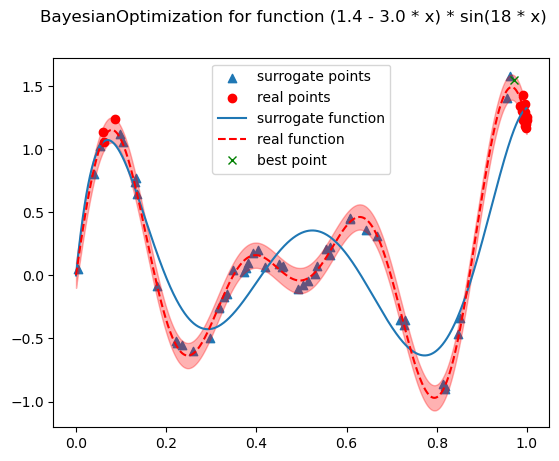
\includegraphics[width=\textwidth]{lab6/imgs/obj2_ucb.png}
        \caption{UCB}
    \end{subfigure}
    \begin{subfigure}{0.5\textwidth}
        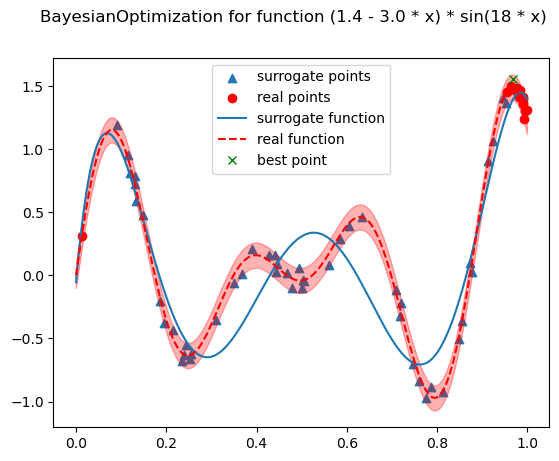
\includegraphics[width=\textwidth]{lab6/imgs/obj2_lcb.png}
        \caption{LCB}
    \end{subfigure} \\
    \begin{subfigure}{0.5\textwidth}
        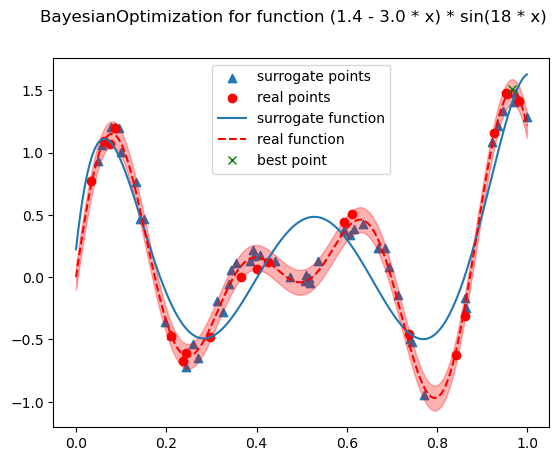
\includegraphics[width=\textwidth]{lab6/imgs/obj2_pi.png}
        \caption{PI}
    \end{subfigure}
    \begin{subfigure}{0.5\textwidth}
        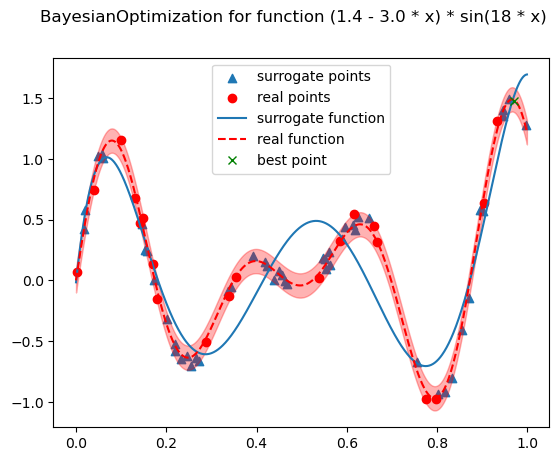
\includegraphics[width=\textwidth]{lab6/imgs/obj2_ei.png}
        \caption{EI}
    \end{subfigure}
    \caption{Objective2 with different acquisition functions}
    \label{fig:bo-acquisition}
\end{figure}
We can see that the acquisition functions have two main behavious: UCB and LCB focus right away on the optimal region while PI and EI are more focused on the exploration of the space.

\paragraph*{Kernel}
\begin{table}[H]
    \centering
    \begin{tabular}{|c|c|c|}
        \textbf{Kernel} & \textbf{Mean}  & \textbf{Std. Deviation} \\\hline
        RBF             & 0.8909, 1.7960 & 0.0500, 0.1031          \\
        DotProduct      & 0.8937, 1.7634 & 0.0399, 0.1153          \\
        ExpSineSquared  & 0.8828, 1.7768 & 0.0599, 0.1307          \\
        \hline
    \end{tabular}
    \caption{Best point found with Objective3 and UCB acquisition function}
    \label{tab:kernel}
\end{table}
The results are roughly the same for all the kernels and all have quite high variance.

\begin{figure}[H]
    \begin{subfigure}{0.5\textwidth}
        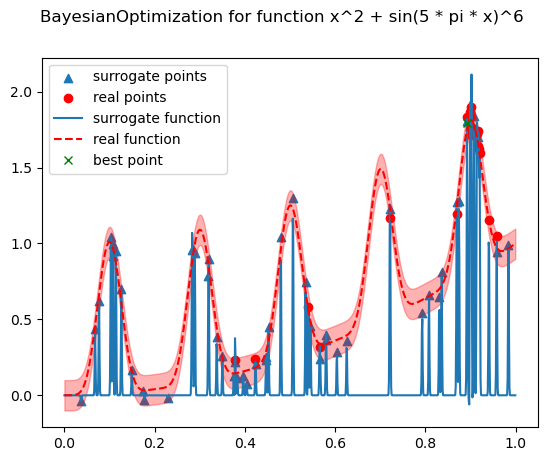
\includegraphics[width=\textwidth]{lab6/imgs/obj3_rbf.png}
        \caption{RBF}
    \end{subfigure}
    \begin{subfigure}{0.5\textwidth}
        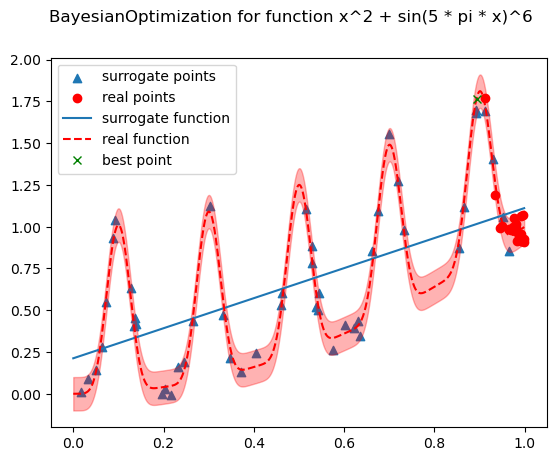
\includegraphics[width=\textwidth]{lab6/imgs/obj3_dot.png}
        \caption{DotProduct}
    \end{subfigure} \\
    \begin{subfigure}{\textwidth}
        \centering
        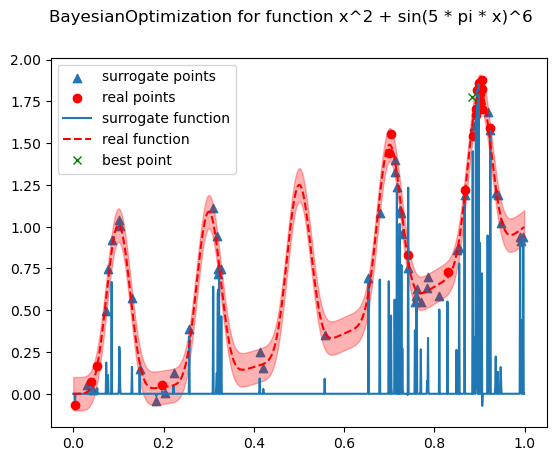
\includegraphics[width=0.5\textwidth]{lab6/imgs/obj3_exp.png}
        \caption{ExpSineSquared}
    \end{subfigure}
    \caption{Objective3 with different kernels}
    \label{fig:bo-kernel}
\end{figure}
We can see that differently than without the kernel, the Gaussian Process in not able to approximate the real function well but the sampled points are still in the optimal region.
